\section{MATLAB Code for RLC Transient Response}
\begin{verbatim}
%% Part 1:
clear

% For the case where R = 100Ohm, C = 6.8nF and L=10mH
R = 100;
C = 6.8E-9;
L = 10E-3;

zeta = R/2 * sqrt(C/L); % approximately 0.0412, so underdamped
w_n = 1/sqrt(L*C);
w_d = w_n * sqrt(1 - zeta^2);

% We know that the circuit is underdamped because zeta < 1

% We obtained C1 = -1, C2 = -(w_n/w_d) * zeta
C1 = -1;
C2 = -(w_n/w_d) * zeta;

t = 0:1E-6:1E-3;
y = exp(-zeta * w_n .* t) .* (C1*cos(w_d.*t) + C2 * sin(w_d.*t)) + 1;
plot(t, y, 'red');

hold on

%% Critically damped

% For the critically damped case:
R = 2 * (1 / sqrt(C/L));
zeta = R/2 * sqrt(C/L);
w_n = 1/sqrt(L*C);

% We obtained that C1 = -1, and C2 = -w_n.
C2 = -w_n;
C1 = -1;
y = (C1*exp(-zeta * w_n .* t) + C2.*t.*exp(-zeta * w_n .* t)) + 1;
plot(t, y, 'blue');

legend({'Underdamped','Critically Damped'},'Location','southwest')

%% Part 3:
clear
close all

R1 = 25;
R2 = 56;
L = 20E-3;
C = 2E-6;
Vin = 16.2;

a2 = R1*L*C;
a1 = R1*R2*C + L;
a0 = R1+R2;

w_n = sqrt(a0 / a2);
zeta = a1 / (2*sqrt(a0 * a2));
K = 1/a0;

iL_p = Vin / (R1 + R2);
C2 = iL_p * (zeta - sqrt(zeta^2 - 1)) / (2 * sqrt(zeta^2 - 1));
C1 = -C2 - iL_p;

% The current over the inductor.
t = 0:1E-6:1E-2;
% It is overdamped.
y = C1 .* exp((-zeta + sqrt(zeta^2 - 1)) .* t .* w_n) + ...
        C2 .* exp((-zeta - sqrt(zeta^2 - 1)) .* t .* w_n) + iL_p;

plot(t, y, "blue", "LineWidth", 2);
ylim([0, 0.3])
legend("Overdamped Behavior")    
\end{verbatim}

\section{Prelab - RLC Frequency Response}
\section{Problem 1: Decibels}
\begin{enumerate}
    \item Given $x(t) = 5 \cos \left(2\pi 1000t\right)$
          \begin{itemize}
              \item What is the amplitude and the $V_{pp}$ of the signal?

                    The amplitude of the signal is $5V$ and the $V_{pp}$ is $2 \cdot 5V = 10V$.
              \item What is the $V_{rms}$ of the signal?

                    The $V_{rms}$ of a sinusoidal signal is given by
                    \begin{equation}
                        V_{rms} = \frac{V_A}{2\sqrt{2}} = \frac{5V}{\sqrt{2}} = 3.535V
                    \end{equation}
              \item What is the amplitude of the spectral peak in dBVrms?
                    The amplitude of the spectral peak in dBVrms is given by the following relation:
                    \begin{equation}
                        A_{dBV_{rms}} = 20 \log_{10} \left(V_{rms}\right) = 20 \log_{10} \left(3.535V\right) = 10.9dBV_{rms}
                    \end{equation}
          \end{itemize}
    \item Given a square wave of $1V_{pp}$ the voltage changes between -0.5V to 0.5V
          \begin{itemize}
              \item What is the signal amplitude in $V_{rms}$?
                    To find the RMS value of a square wave, the following relation is used:
                    \begin{equation}
                        V_{rms} = \sqrt{\frac{1}{T}\left[\int_{0}^{T}f(t)^2 dt\right]}
                    \end{equation}
                    The square wave can be specified as a piecewise function:
                    \begin{equation}
                        f(t) = \begin{cases}
                            -0.5 & \text{if } 0 \leq t \leq \frac{T}{2} \\
                            0.5  & \text{if } \frac{T}{2} \leq t \leq T
                        \end{cases}
                    \end{equation}
                    Performing the integral over the function,
                    \begin{equation}
                        \begin{gathered}
                            V_{rms} = \sqrt{\frac{1}{T}\left[
                                    \int_{0}^{T/2}(-0.5)^2 dt
                                    +
                                    \int_{T/2}^{T}(0.5)^2 dt
                                    \right]} \\
                            = \sqrt{0.25 \cdot \frac{1}{T}\left(\frac{T}{2} + T - \frac{T}{2}\right)} \\
                            = \sqrt{0.25}V \\
                            = 0.5V
                        \end{gathered}
                    \end{equation}
              \item What is the amplitude in dBVrms?
                    \begin{equation}
                        V_{dB_{rms}} = 20\log_{10}\left(V_{rms}\right) = 20\log_{10}\left(0.5V\right) = -6.02dBV_{rms}
                    \end{equation}
          \end{itemize}
\end{enumerate}
\section{Problem 2: Determination of Fourier Series Coefficients}
\begin{enumerate}
    \item Determine the Fourier series coefficients up to the 5th harmonic of the function $f(t) = 4t^2$

          To determine the fourier series coefficients, first recognize that the function is an even function by the very fact that it is a polynomial of an even degree. Knowing this, the relations used to compute the fourier series coefficients are:
          \begin{equation}
              \begin{gathered}
                  a_n = \frac{4}{T}\int_{-T}^{T}t^2 \cos(n\omega_0t) dt \\
                  a_0 = \frac{1}{T}\int_{0}^{T}t^2 dt \\
                  b_n = 0 \\
              \end{gathered}
          \end{equation}
          Where it is known that $T = 1$ due to the interval being given as $[-0.5, 0.5]$. Furthermore, $\omega_0 = \frac{2\pi}{T} = 2\pi$. By using the help of an integration table, the integral for $a_n$ is
          \begin{equation}
              a_n = 4\cdot \left[
                  \frac{2t \cos(n\omega_0t)}{4\pi^2n^2} + \frac{n^24\pi^2 - 2}{8\pi^3n^3}sin(n\omega_0t)
                  \right]_{-T}^{T}
          \end{equation}

          Evaluating this integral:
          \begin{equation}
              a_n = 4 \cdot \left(\frac{4 \cdot (-1)^n}{4\pi^2n^2}\right)
              = \frac{4 \cdot (-1)^n}{\pi^2n^2}
          \end{equation}

          For $a_0$, the integral is straightforward:
          \begin{equation}
              a_0 = \frac{1}{T}\int_{0}^{T}t^2 dt = \left[\frac{t^3}{3}\right]_{0}^{T} = \frac{1}{3}
          \end{equation}

          So the first five coefficients are:
          \begin{equation}
              a_n = \left\{ \frac{-4}{\pi^2}, \frac{4}{16\pi^2}, \frac{-4}{36\pi^2}, \frac{4}{64\pi^2}, \frac{-4}{100\pi^2} \right\}
          \end{equation}
    \item Use MATLAB to plot the original function and the inverse Fourier transform. Put both graphs into the same diagram.
          \begin{figure}[H]
              \centering
              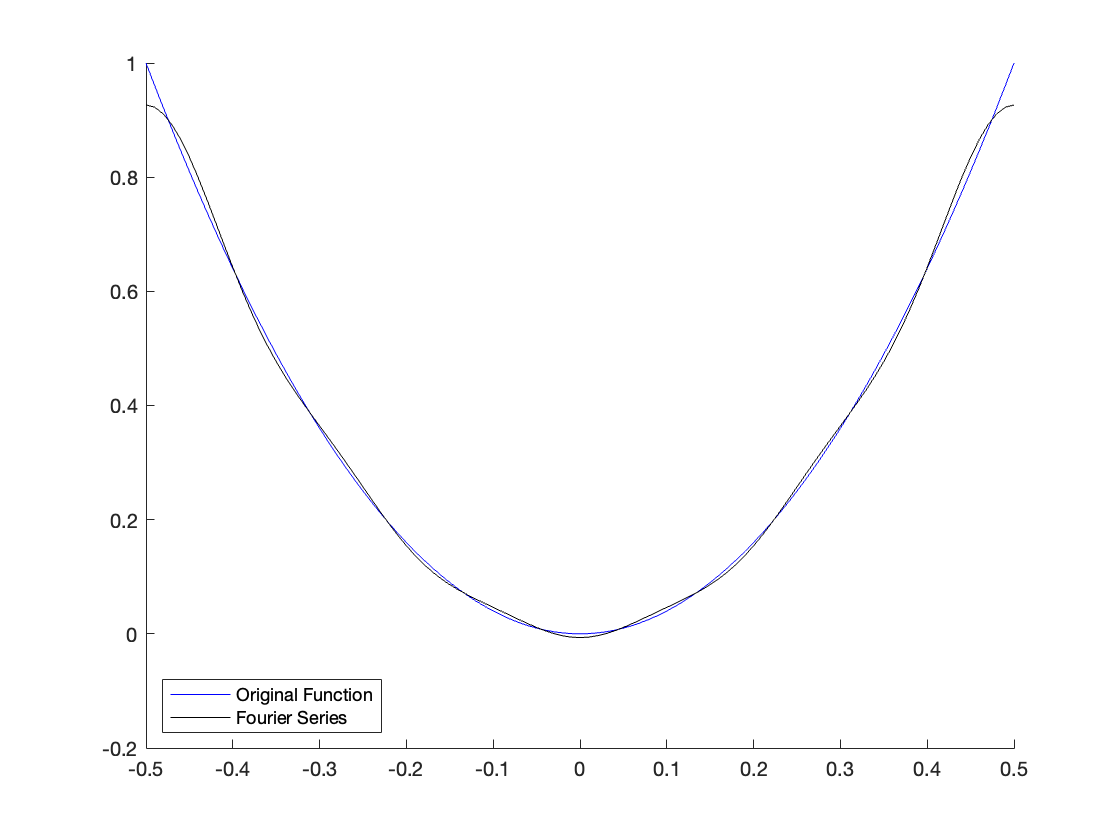
\includegraphics[width=0.8\textwidth]{images/prelab_problem_2_plot.png}
              \caption{The plot of the original function, its inverse fourier transform, the fourier series representation up to the fifth harmonic, and the representation's inverse fourier transform}
          \end{figure}
          The code used:
          \begin{verbatim}
t = -0.5:0.01:0.5;
f = 4*t.^2;
f_fs = 1/3;

% Fourier series representation of the function
for i=1:5
    % w_0 = 2pi
    % T = 1
    a_i = (4*(-1)^i)/(pi^2*i^2);
    f_fs = f_fs + (a_i .* cos(i.*2.*pi.*t));
end
hold on

plot(t, f, "blue");
plot(t, f_fs, "black");
xlim([-0.5, 0.5]);

plot(t, abs(ifft(f)), "red");
plot(t, abs(ifft(f_fs)), "green");

legend({"Original Function", ...
    "Fourier Series Representation", ...
    "IFFT", ...
    "IFFT of Fourier Series" ...
    }, "Location", "southwest")
          \end{verbatim}
\end{enumerate}

\newpage
\section{Problem 3: FFT of a Rectangular Wave}

\begin{figure}[H]
    \centering
    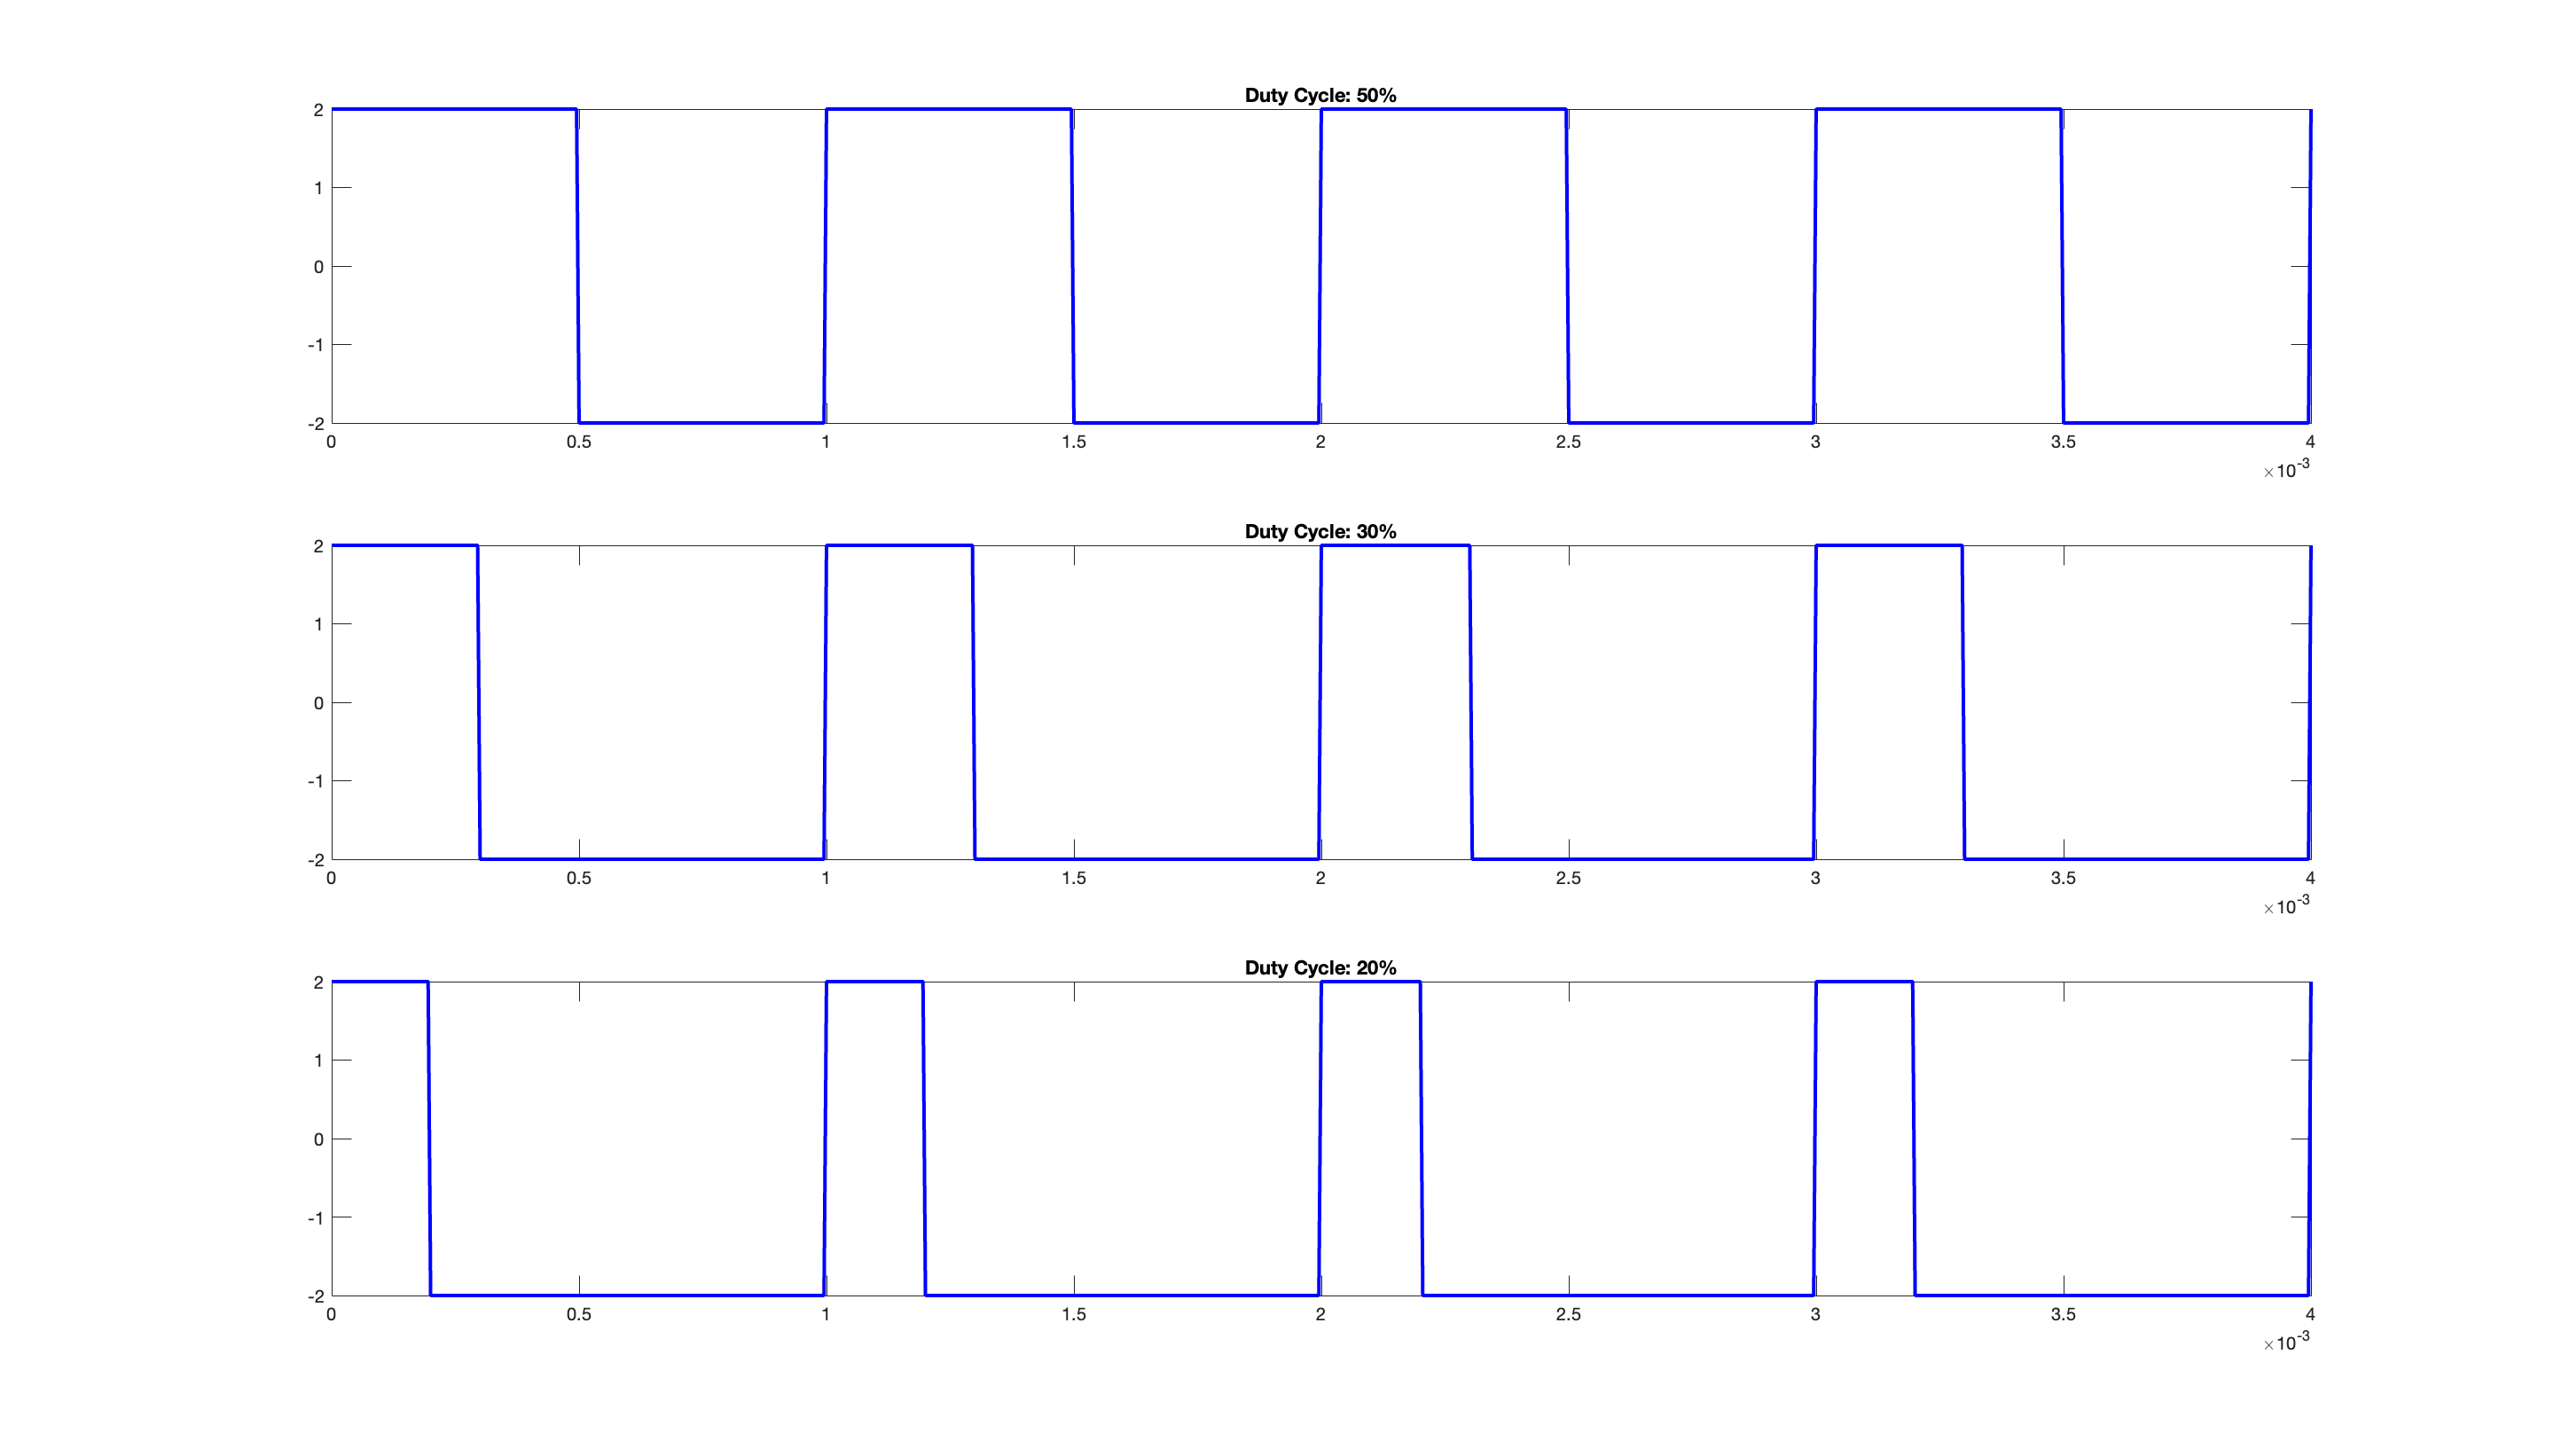
\includegraphics[width=0.8\textwidth]{images/prelab_problem_3_time.png}
    \caption{A figure showing the different rectangular waves based on their duty cycles. Plotted using MATLAB.}
\end{figure}

\begin{figure}[H]
    \centering
    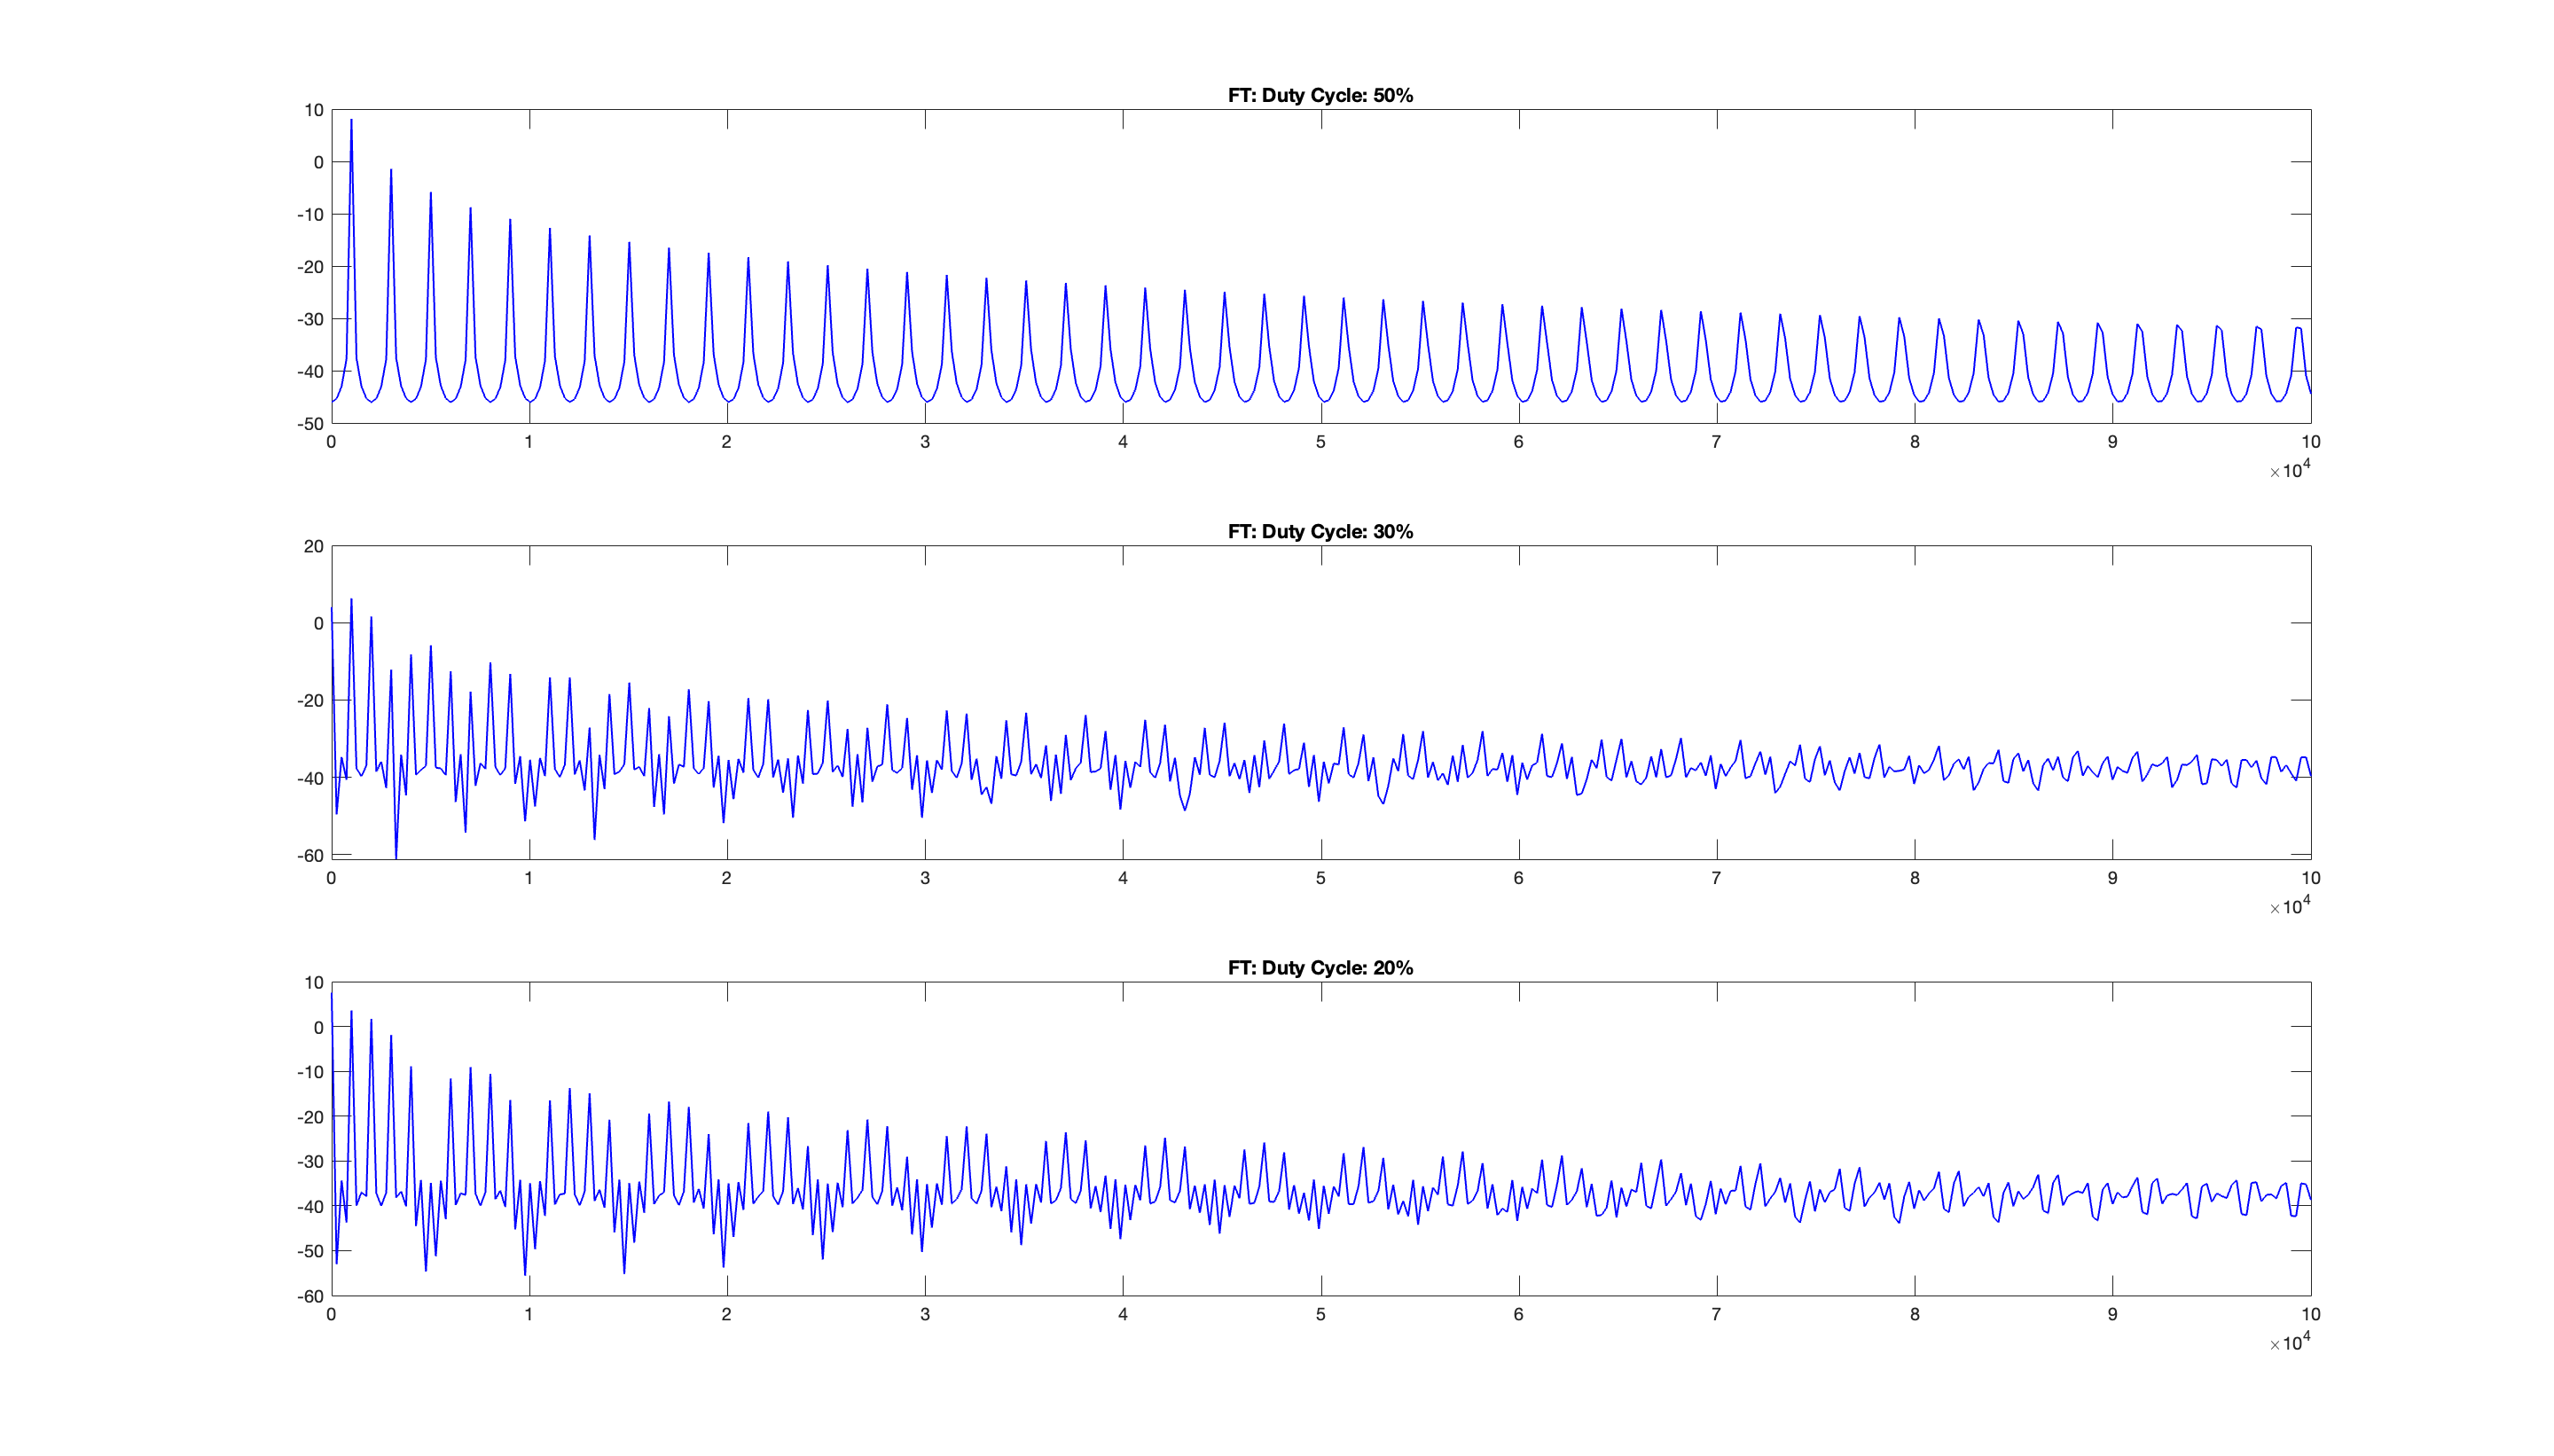
\includegraphics[width=0.8\textwidth]{images/prelab_problem_3_freq.png}
    \caption{A figure showing the different rectangular waves' spectra based on their duty cycles. Plotted using MATLAB.}
\end{figure}

The code used to plot the figures:
\newpage
\begin{verbatim}
%% Time plots

[t_fifty, signal_fifty, f_fifty, y_fifty] = get_square(50);
[t_thirty, signal_thirty, f_thirty, y_thirty] = get_square(30);
[t_twenty, signal_twenty, f_twenty, y_twenty] = get_square(20);

subplot(3, 1, 1);
plot(t_fifty, signal_fifty, "blue", "LineWidth", 2);
title("Duty Cycle: 50%");

subplot(3, 1, 2);
plot(t_thirty, signal_thirty, "blue", "LineWidth", 2);
title("Duty Cycle: 30%");

subplot(3, 1, 3);
plot(t_twenty, signal_twenty, "blue", "LineWidth", 2);
title("Duty Cycle: 20%");

%% Frequency plots
subplot(3, 1, 1);
plot(f_fifty, y_fifty, "blue", "LineWidth", 1);
title("FT: Duty Cycle: 50%");


subplot(3, 1, 2);
plot(f_thirty, y_thirty, "blue", "LineWidth", 1);
title("FT: Duty Cycle: 30%");


subplot(3, 1, 3);
plot(f_twenty, y_twenty, "blue", "LineWidth", 1);
title("FT: Duty Cycle: 20%");
\end{verbatim}
Where the function \texttt{get\_square} is defined as:
\newpage
\begin{verbatim}
function [t, signal, f, y_single_db] = get_square(duty_cycle)
    period = 1e-3;
    Fs = 200e3;
    frequency = 1/period;
    Vpp = 2;
    duration = period * 4;
    
    % The signal
    t = 0:1/Fs:duration;
    signal = Vpp*square((2*pi*frequency)*t, duty_cycle);
    plot(t, signal, "blue", "LineWidth", 2);
    
    % The fourier transform of the signal
    rms_value = sqrt(mean(signal.^2));
    N = length(signal); % The length of the signal
    
    y = fft(signal, N);
    y_mag = 2*(abs(y)/N); % Magnitudes of y
    
    y_single = y_mag(1:floor(N/2)) * 2;
    f_nyquist = Fs / 2;
    
    y_single_db = 20*log10(y_single / rms_value);
    f = linspace(0, f_nyquist, length(y_single));
end
\end{verbatim}

Following by the equation:

\begin{equation}
    c_k = \frac{1}{k\pi}\sin(k\omega_0T_1)
\end{equation}

It is observed that for a lower $T_1$, for each frequency component the amplitude of the component is lower. This is due to the fact that the pulse width is lower, and thus the signal is more spread out in the time domain. This is also observed in the frequency domain, where the frequency components are more spread out, thereby more frequency components are required to represent the signal.

\section{Problem 4: FFT of an audio file}

\begin{figure}[H]
    \centering
    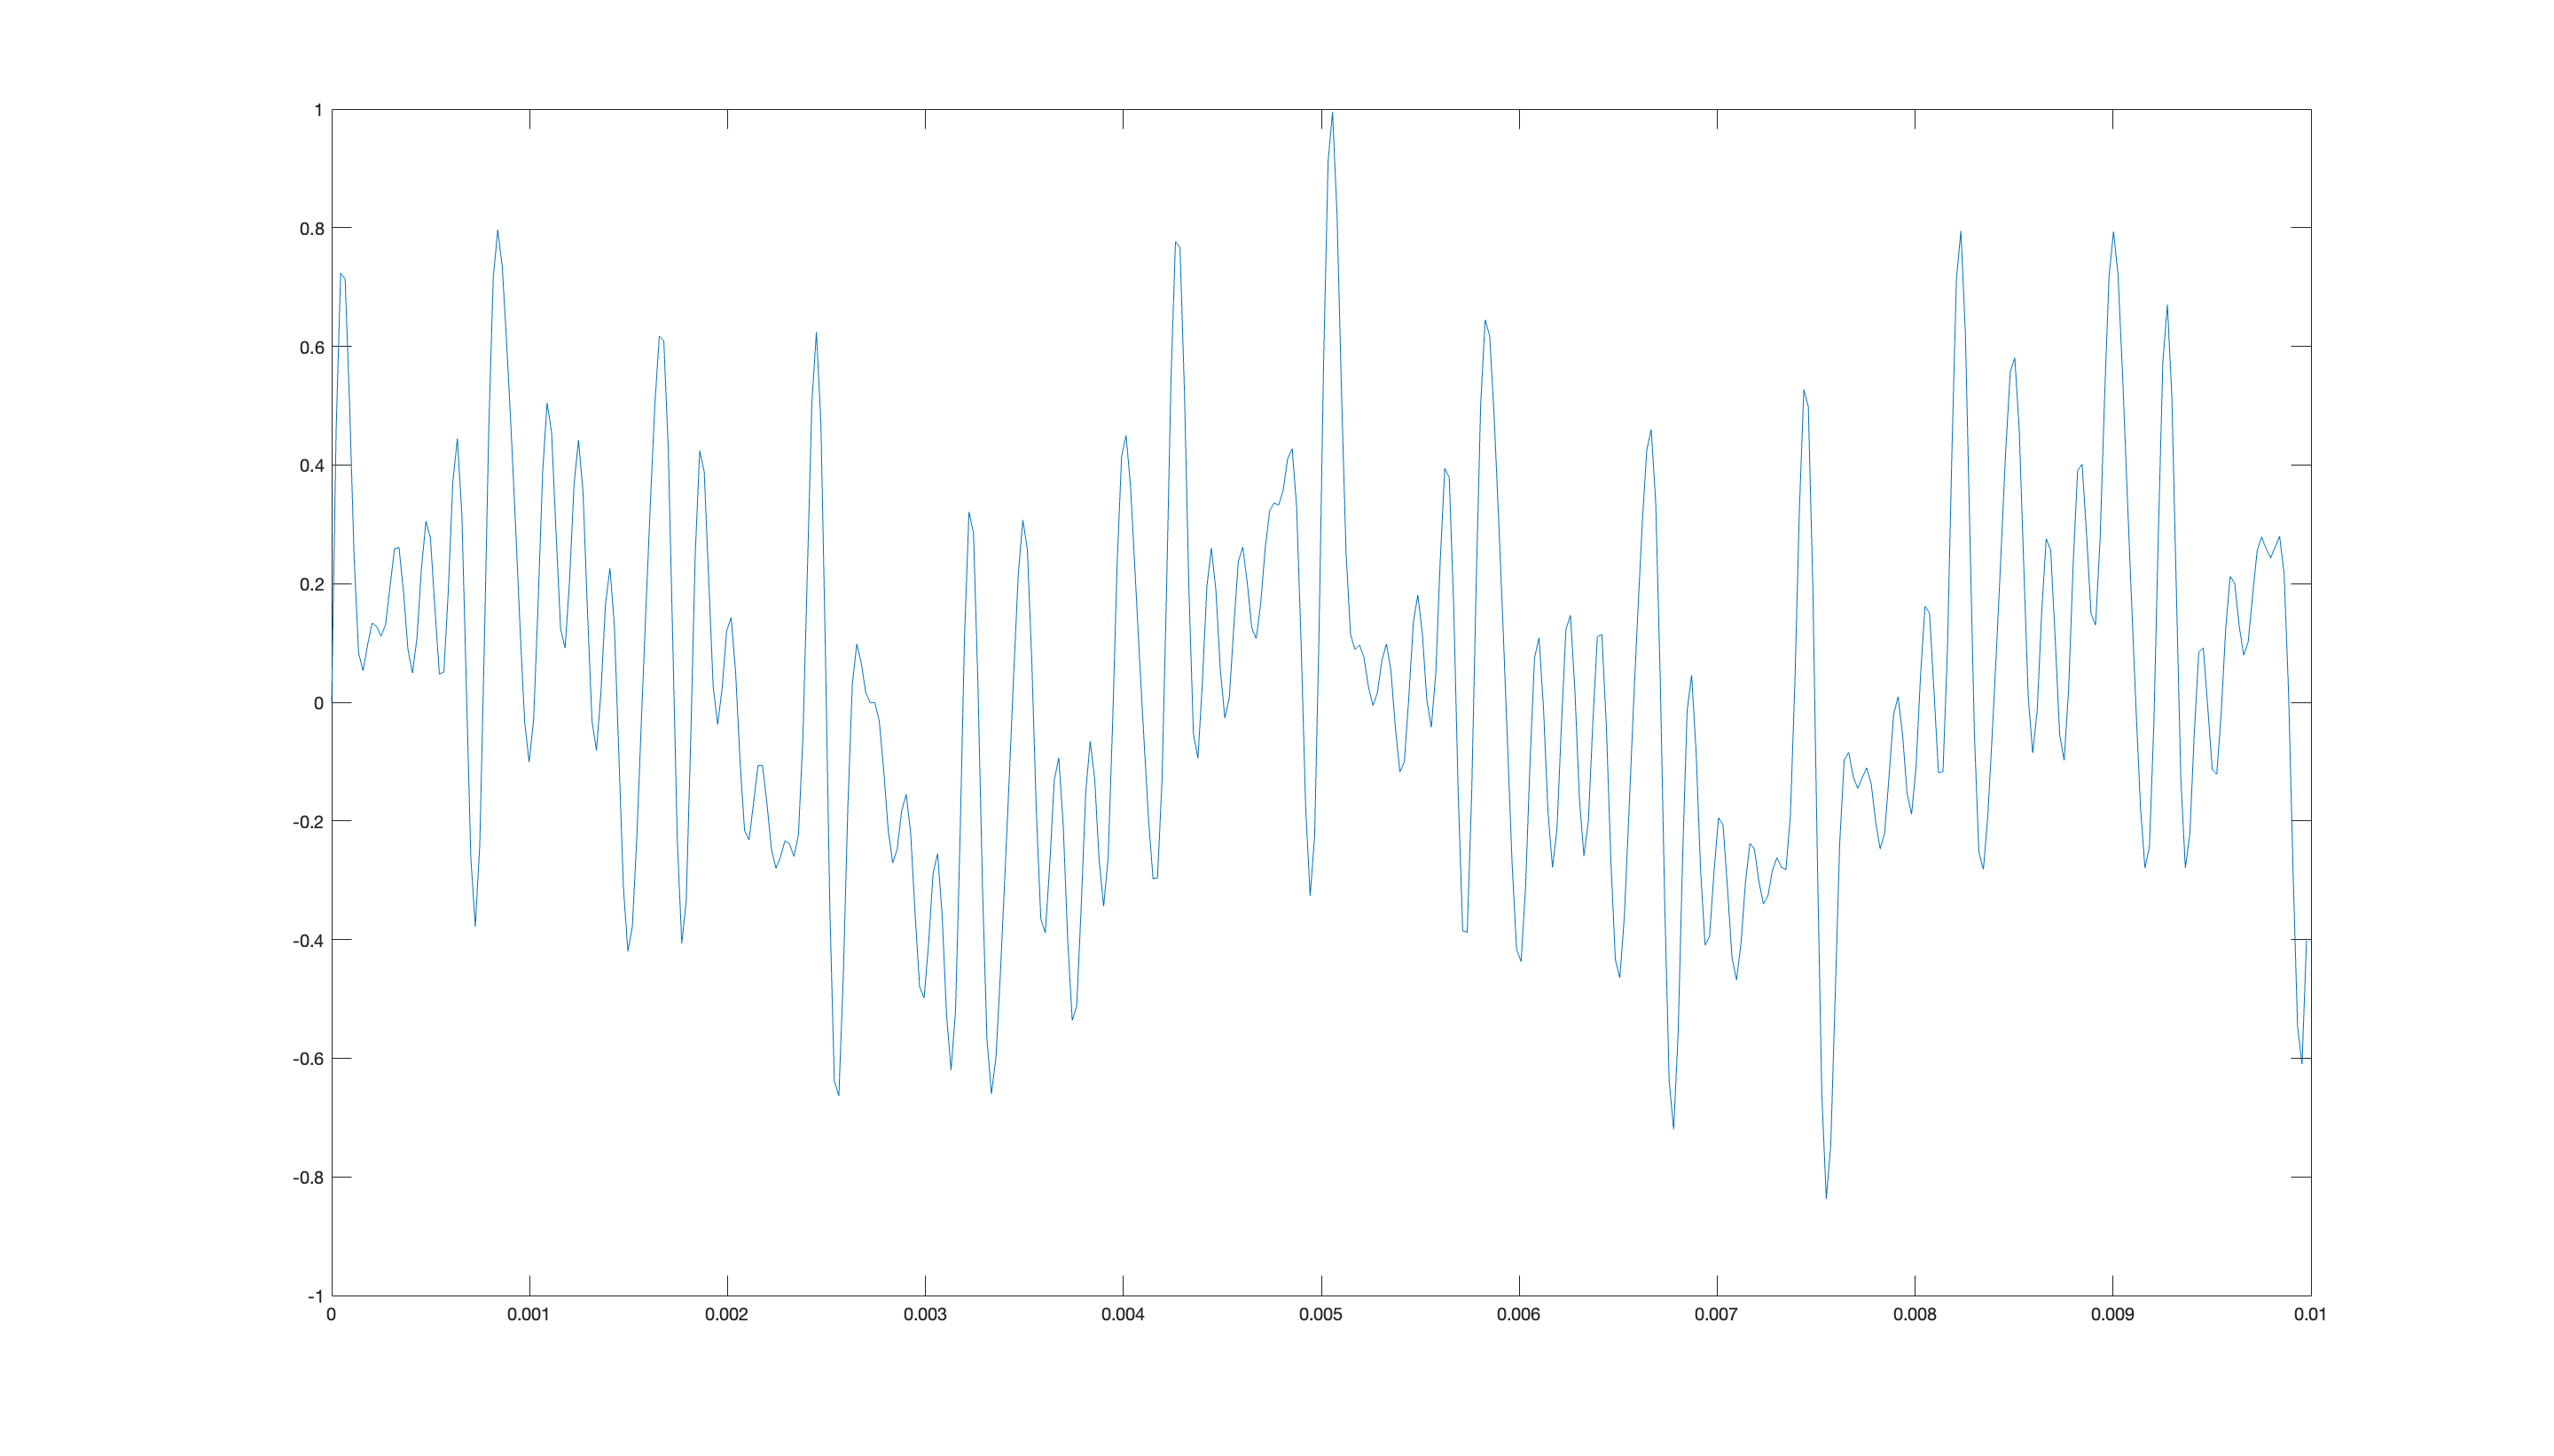
\includegraphics[width=0.8\textwidth]{images/prelab_problem_4_time.png}
    \caption{A figure showing the plot of the audio file}
\end{figure}
\begin{figure}[H]
    \centering
    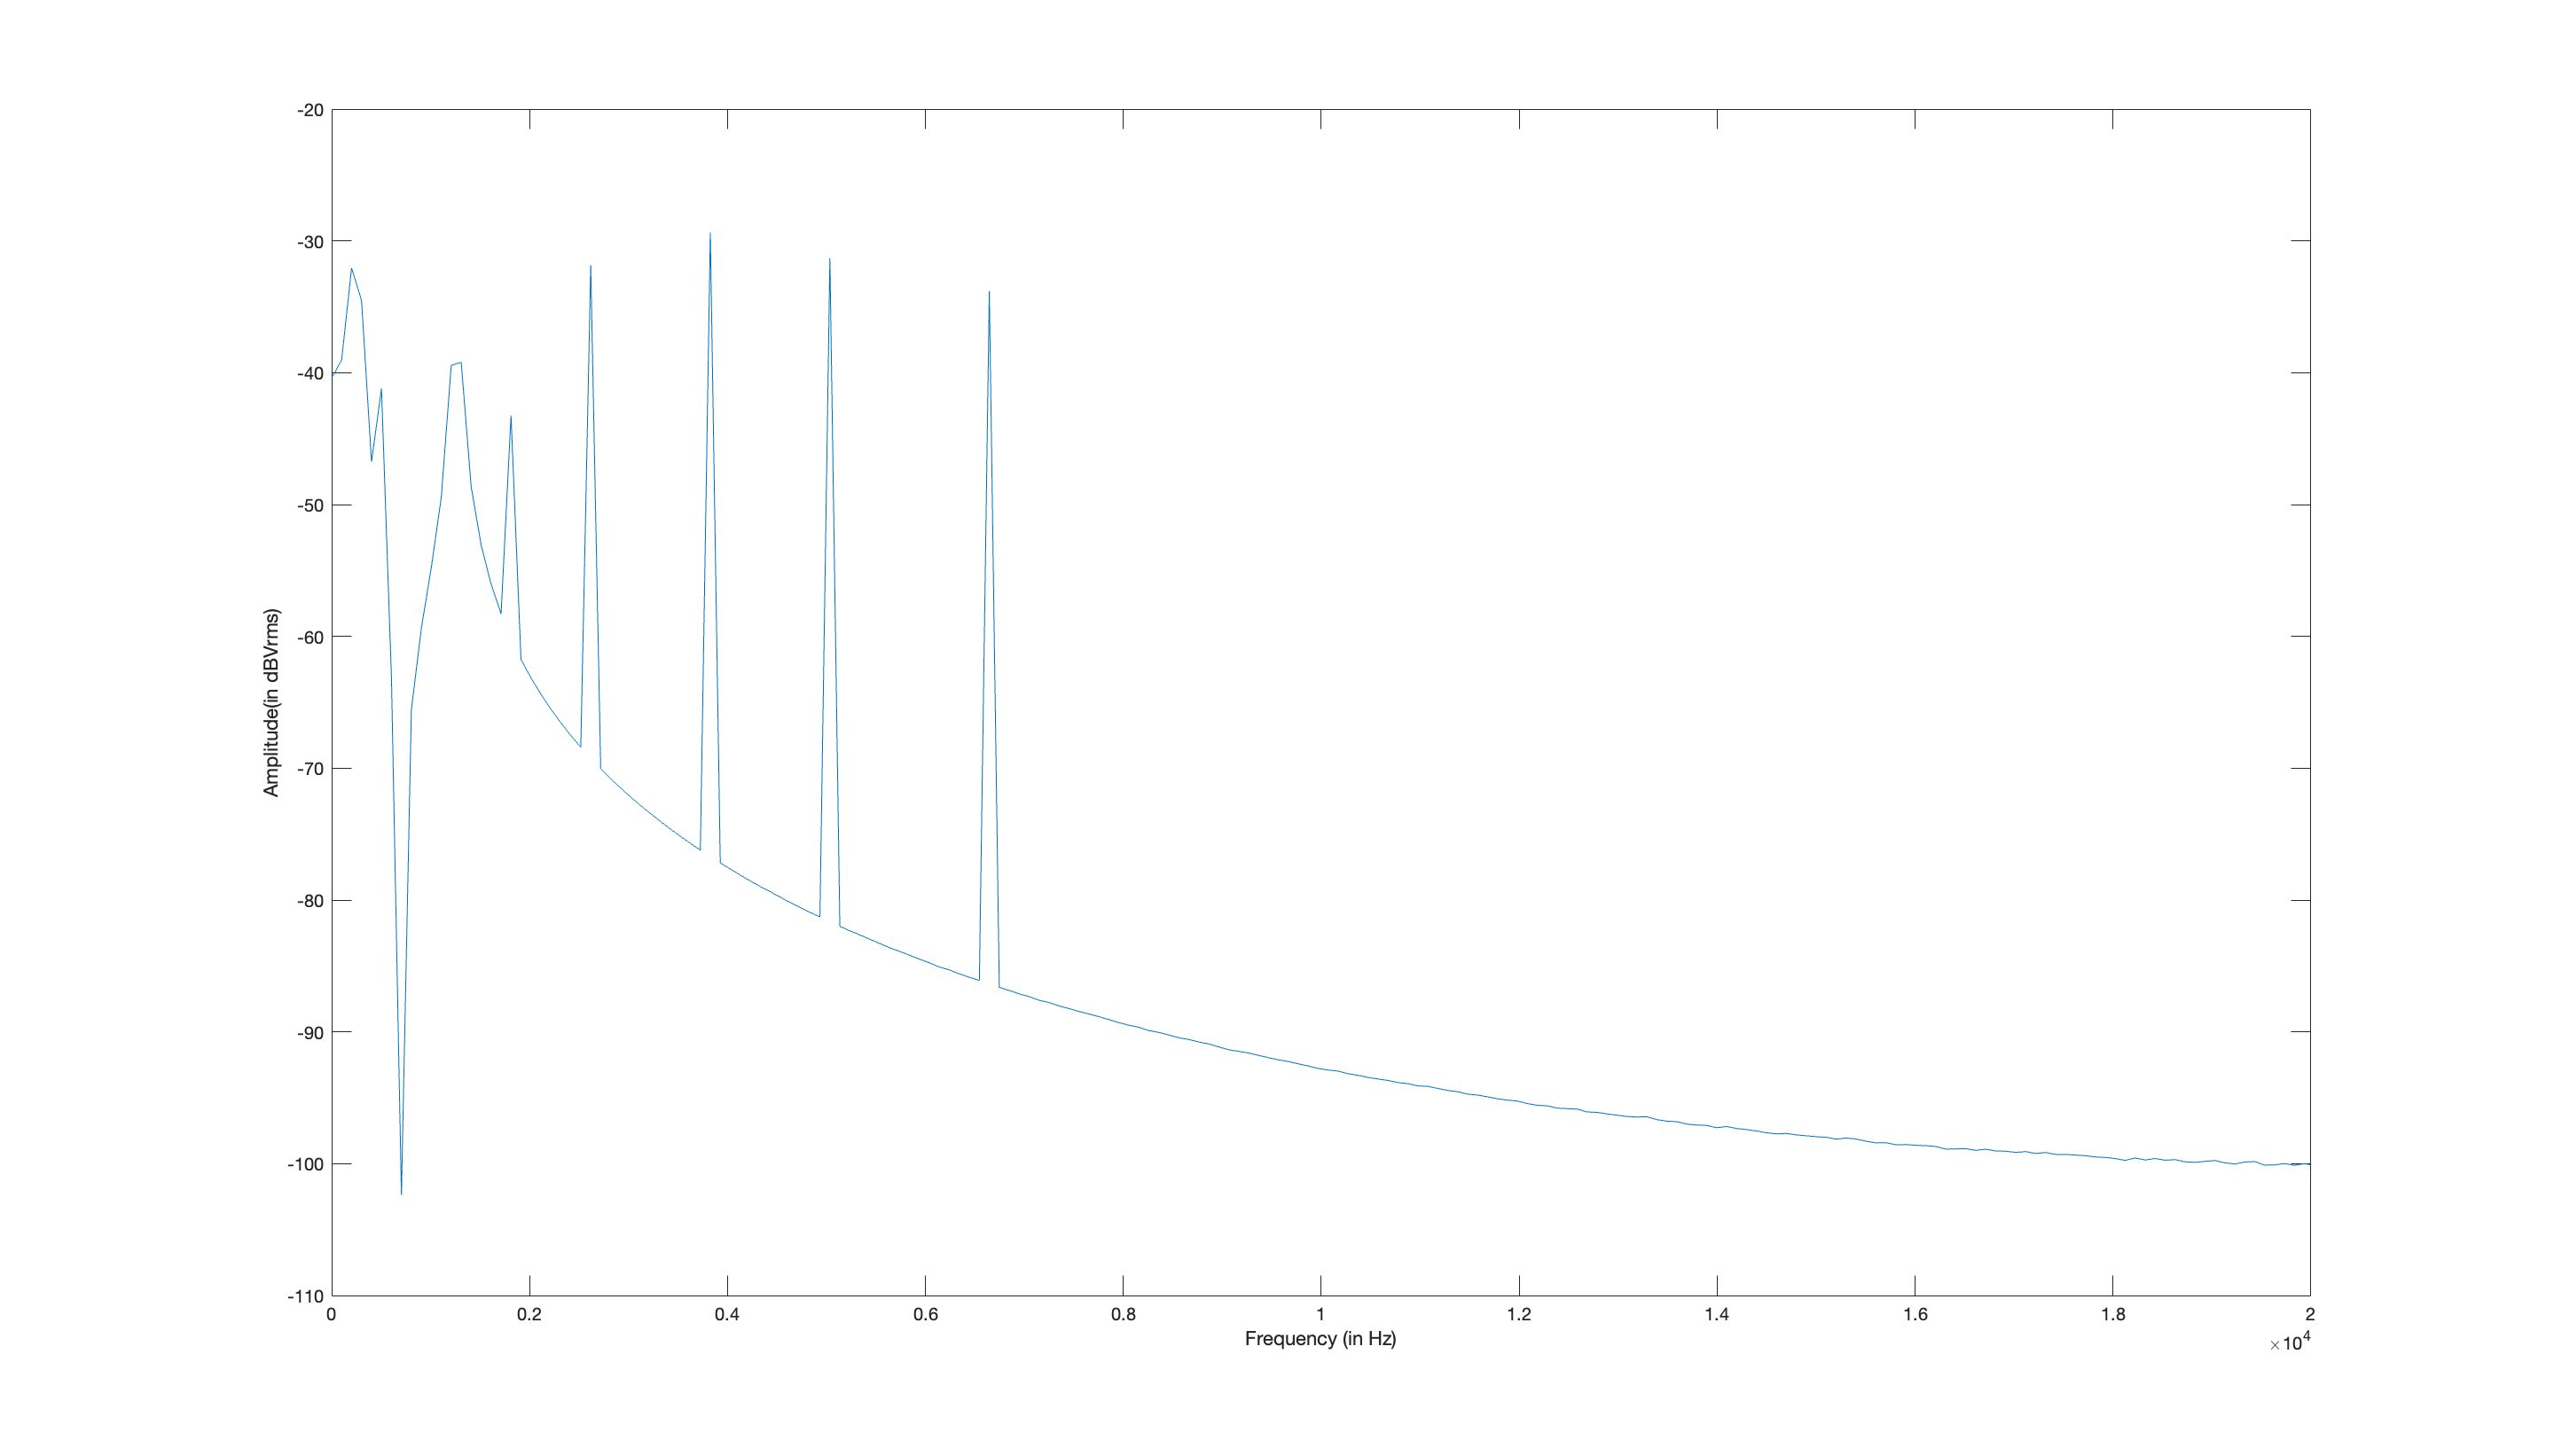
\includegraphics[width=0.8\textwidth]{images/prelab_problem_4_freq.png}
    \caption{A figure showing the frequency spectrum of the audio file}
\end{figure}

The following code was used for the plots:
\vspace{1cm}
\begin{verbatim}
%% Problem 4:
[y, Fs] = audioread("s_samp.wav");

N_samples = Fs * 10E-3;
y = y(1:N_samples);
t = 0:1/Fs:((10E-3)-1/Fs);
plot(t, y);
%% 
Y = fft(y);
rms = sqrt(mean(abs(Y.^2)));

Fs_nyquist = Fs / 2; 

Y_single = 2 * abs(Y) / N_samples;
Y_single = Y_single(1:floor(N_samples/2));
f = linspace(0,Fs_nyquist,length(Y_single));
Y_db = 20*log10(Y_single ./ rms);

plot(f, Y_db);
ylabel("Amplitude(in dBVrms)")
xlabel("Frequency (in Hz)");
xlim([0, 20000]);
\end{verbatim}

The following tones are observed:
\begin{itemize}
    \item G3 - 201Hz
    \item B4 - 503Hz
    \item E6 - 1308Hz
    \item A6 - 1812Hz
    \item E7 - 2617Hz
    \item A\#7 - 3826Hz
    \item D\#8 - 5034Hz
    \item G\#8 - 6645Hz
\end{itemize}